\documentclass[12pt]{article}
\usepackage[utf8]{inputenc}
\usepackage{amsmath}
\usepackage{graphicx}
\usepackage{listings} % for source code inserts
\title{CS 470 Spring 2011 \\
     Project 3}
\author{Colby Blair}
\date{Due April 27th, 2011}
\begin{document}
\maketitle

\begin{abstract}
Fuzzy Controls are a very useful in Artificial Intelligence. They don't resemble intelligence, in that they are
fairly static. They don't learn, and only react to inputs in the way originally intended by the programmer.
They are, however, very useful. They are best used in environments with set inputs, and the corresponding
outputs are imperical values, besides some scaling. 

Fuzzy control systems are also much simplier, and respond much better to specific problems. Therefore, 
their structure can tell us much more about the solutions than more complicated AI solutions, like Artificial
Neural Networks. Fuzzy control system also give us great training or teaching algorithms, in which to teach
other methods of AI.
\end{abstract}

\thispagestyle{empty}

\pagebreak

\thispagestyle{empty}
\tableofcontents
\listoffigures

\pagebreak

\setcounter{page}{1}

\section{Introduction}
Fuzzy control systems are a more imperical way of implementing AI. This project will demonstrate a simple 
fuzzy control system, while trying to land a moon lander. Fuzzy control systems try to create actions by
quantifying inputs. And example for the lander goes: "if high and descending slow, then burn low", where 
burn is the engines output. A fuzzy system could be made of as many of these rules as one could think of,
but a better approach is to create functions that produce the same outputs.

The lander works in environments of varying gravity and wind. To complicate things, the lander has a narrow 
landing pad to land on. Controls must be fairly tight, but also dynamic to handle many changing environment 
inputs. The challenge then is that we must quantify the inputs, like 'high'. What is high? Is it either true or 
false? Probably not. 'High' is probably then a value from 0 to 100, or in our case, 0.0000 to 1.0000. The lander 
can adjust its burn accordingly, so that more burn is outputed closer to landing. 

To get useful outputs from a fuzzy control system, there are 3 steps:
\begin{enumerate}
	\item fuzzify inputs
	\item select fuzzy inputs by applying fuzzy logic
	\item defuzzify fuzzy logic output
\end{enumerate}

\subsection{Fuzzify Inputs}
There has already been a few rules defined now, like "if high and descending slow, then burn low" and 
"if low and descending medium, then burn medium" . This is generalized with some basic fuzzifycation:

\begin{figure}[h]
        \begin{center}
                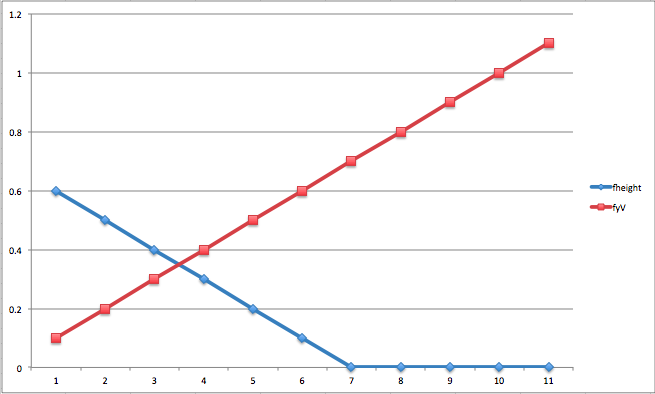
\includegraphics[width=90mm]{report_images/ex_burn.png}
                \caption{An example y axis fuzzification}
                \label{ex_burn}
        \end{center}
\end{figure}

The lander still needs to consider x axis controls, but Figure \ref{ex_burn} gives an example of y control that
is somewhat similar to the actual findings in this report. 

\subsection{Apply Fuzzy Logic}
In general, fuzzy logic has two operators considered
here: $OR$ and $AND$:

\begin{tabular}{r l}
	$a AND b$		&	$ = min(a,b) $ \\
	$a OR b$		&	$ = max(a,b) $ \\
	$where$		&	\\
				&	$a,b$ are fuzzified values
\end{tabular}

\subsection{Defuzzify Fuzzy Logic}
Defuzzification means to turn our fuzzy logic back into real world values, or useful output. There are several 
methods to defuzzify our fuzzy logic, including scaling and centroid operations. In this report, the simple 
method of scaling does fine.

\pagebreak

\section{Moon Lander}
The lander this report uses must be a lander for more than just earth's moon, because random wind gusts 
exists. Since the x and y forces are completely perpendicular, from physics it is known that the forces are
independent. We then have two independent, x and y, controls.

\begin{figure}[h!]
        \begin{center}
                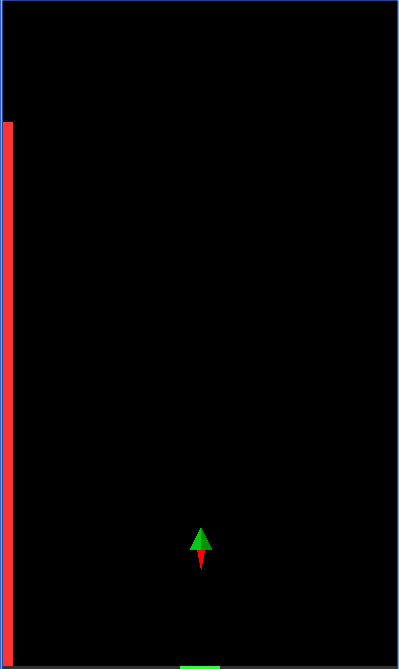
\includegraphics[width=30mm]{report_images/simple_flight.png}
                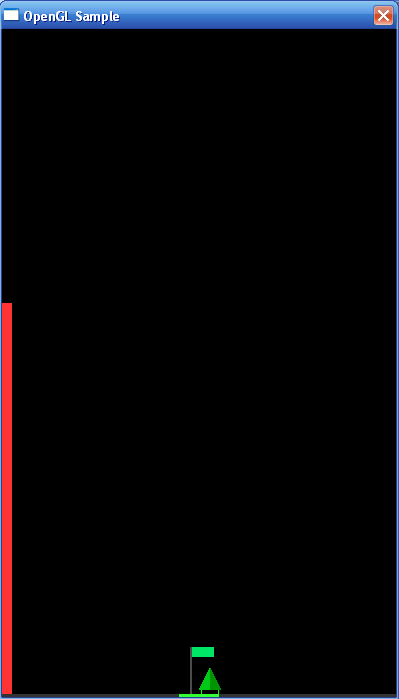
\includegraphics[width=30mm]{report_images/simple_landing.png}
                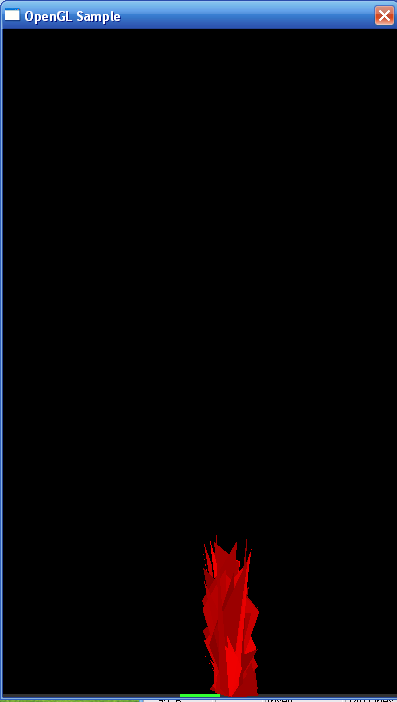
\includegraphics[width=30mm]{report_images/crash.png}
                \caption{The moon lander}
                \label{simple}
        \end{center}
\end{figure}

\subsection{Fuzzify Inputs}
The fuzzifications are actually fairly simple. That said, they did the job well enough to land the lander 
over 90% of the time. With this, not much more improvement was put into the current system.

\subsubsection{Y}
The y fuzzy velocity algorithm is as follows:

\begin{tabular}{r l}
	$f_{v_y}(V_y)$	&	$ = 0 $ if $ V_y < V_{y max} $ \\
				&	$ = 1 $ if  $ V_y > V_{y max} + k_1 $ \\
				& \\
 				&	$ = \frac{1 - (V_{y max} - V_y)}{V_{y max}} $ otherwise\\
	where		& \\
				& $k_1 = 3$
\end{tabular} \\

The y fuzzy height algorithm is as follows:

\begin{tabular}{r l}
	$f_{y}(y)$		&	$ = 0 $ if $ y > y_{cutoff} $ \\
				& \\
 				&	$ = \frac{(Y_{max} - y)}{Y_{max}} - k_2$ otherwise\\
	where		& \\
				& $y_{cutoff} = 50$ \\
				& $k_2 = .4$ \\
\end{tabular} \\

The resulting fuzzifications outputs are:

\begin{figure}[h!]
        \begin{center}
                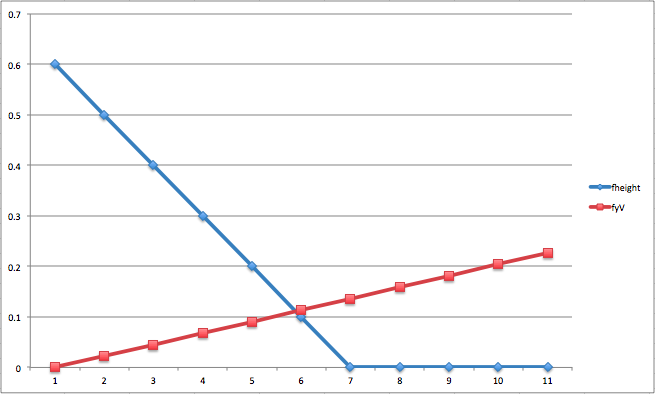
\includegraphics[width=80mm]{report_images/yfuzzy.png}
                \caption{Y input fuzzifications}
                \label{yfuzzy}
        \end{center}
\end{figure}

\subsubsection{X}
X values were very simple, since they stayed relatively low (0.0 - 2.0).  The y fuzzy velolcity algorithm is as
follows: \\

\begin{tabular}{r l}
	$f_{V_x}(V_x)$	&	$ = \frac{1 - (V_{x max} - V_x)}{V_{x max}} $\\
	where		&	\\
				&	$V_{x max} = 5.0$\\			
\end{tabular} \\

The x fuzzy position algorithm is as
follows: \\

\begin{tabular}{r l}
	$f_{x}(x)$		&	$ = \frac{1 - (X_{max} - x)}{X_{max}} $\\				
	where		&	\\
				&	$V_{x max} = 2.0$\\	
\end{tabular} \\

The resulting fuzzifications outputs are:

\begin{figure}[h!]
        \begin{center}
                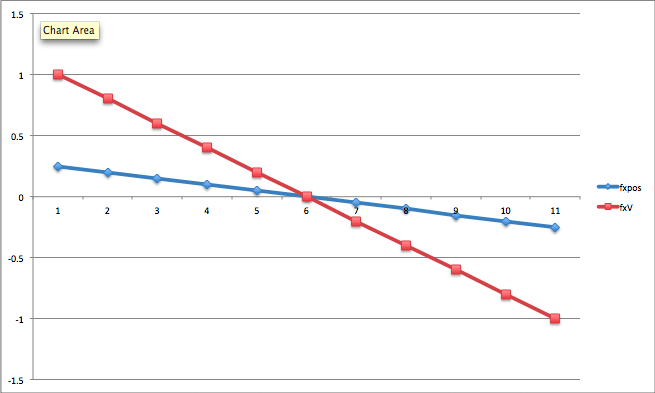
\includegraphics[width=80mm]{report_images/xfuzzy.png}
                \caption{X input fuzzifications}
                \label{xfuzzy}
        \end{center}
\end{figure}

\subsection{Apply Fuzzy Logic}
For selecting fuzzy y values, the $OR$ fuzzy operator was used. For example, this effectively picked 
$max(f_{v_y}(V_y),f_{y}(y)$ from Figure \ref{yfuzzy}. Picking the max values implies that over estimation of
action should result. This is common with scenarios like safety, where under estimation can be chatistrophic.
In the case of the moonlander, this is true.

\subsubsection{Y}
For selecting fuzzy y values, the $OR$ fuzzy operator was used.  The resulting values from the figure are: \\

\begin{tabular}{|c|c|}
	\hline
	$f_{v_y}(V_y)$	&	$f_{y}(y)$		\\
	\hline
	0.6			&	0			\\
	0.5			&	0.022727273	\\
	0.4			&	0.045454545	\\
	0.3			&	0.068181818	\\
	0.2			&	0.090909091	\\
	0.1			&	0.113636364	\\
	0			&	0.136363636	\\
	0			&	0.159090909	\\
	0			&	0.181818182	\\
	0			&	0.204545455	\\
	0			&	0.227272727	\\
	\hline
\end{tabular}

\subsubsection{X}
For selecting fuzzy y values, the $OR$ fuzzy operator was used on the absolute values, since posotive or 
negative values represented left or right movement. The resulting values from the figure are: \\

\begin{tabular}{|c|c|}
	\hline
	$f_{v_x}(V_x)$	&	$f_{x}(x)$		\\
	\hline
	0.25		&	1		\\
	0.2		&	0.8		\\
	0.15		&	0.6		\\
	0.1		&	0.4		\\
	0.05		&	0.2		\\
	0		&	0		\\
	-0.05	&	-0.2		\\
	-0.1		&	-0.4		\\
	-0.15	&	-0.6		\\
	-0.2		&	-0.8		\\
	-0.25	&	-1		\\
	\hline
\end{tabular}

\subsection{Defuzzified Fuzzy Logic}
\subsubsection{Y}
For y values, the defuzzified values needed to be relative to gravity. In low gravity, ouput should be lower 
than in heavy gravity. Gravity cannot be directly measures, but higher gravity will create higher y velocities,
despite our output. This is a loose way of calculating gravity, so y velocity is used to defuzzify the fuzzy 
logic.

The defuzzification algorithm for y velocity is as follows:\\

\begin{tabular}{r l}
	$df_{V_y}(V_y)$	&	$ = f_{v_y}(V_y) * V_y $ \\		
\end{tabular} \\

The defuzzification algorithm for height is as follows:\\

\begin{tabular}{r l}
	$df_{y}(y)$		&	$ = f_{y}(y) * V_y  * k_3$ \\
	where		& \\
				&	$k_3 = .8$
\end{tabular} \\

\subsubsection{X}
For x values, the defuzzified values can be scaled similarly to y values by using x velocity.

The defuzzification algorithm for x velocity is as follows:\\

\begin{tabular}{r l}
	$df_{V_x}(V_x)$	&	$ = f_{v_x}(V_x) * V_x * k_4 $ \\		
	where		& \\
				&	$k_4 = .9$
\end{tabular} \\

The defuzzification algorithm for x position is as follows:\\

\begin{tabular}{r l}
	$df_{x}(x)$		&	$ = f_{x}(x) * V_x  * k_5$ \\
	where		& \\
				&	$k_5 = 1.8$
\end{tabular} \\

\pagebreak


\section{Conclusion}
In conclusion, a fuzzy control system was extremely useful. It was able to perform very well in what is 
probably very simplified test cases. But more importantly, its fuzzification and defuzzified output teaches 
the observer much about the solution of the problem, compared to other AI methods. In this report, none of
the original outputs were changed, even though they may have been extreme.

Perhaps the best function the fuzzy controls provide is a teaching/training algorithm for other AI methods,
like Artificial Neural Networks. Fuzzy controls worked well here, but may fall apart in more extreme 
environments. Teaching an ANN from a fuzzy control could create a base for the ANN to start from,
and the ANN could then generalize the solution to work in more complicated environments.


\section{Results}
The selection of mins and maxs can be best seen in some output from actual runs. The results are pretty 
interesting (all are successful landing unless notified as crash).

\subsection{Review/Summary}
The system worked very well. It landed over 90% of the time, despite its fuzzification simplicity. All crashes
were because of thrust (x output) errors. This could be because of inaccuracies in the x controls, or could
be because of the extreme changes of wind during flight. 

Notice that over corrections were the only irregularity in y control. This comes from selecting the max 
fuzzy value, or using the $OR$ operator. This defaults on caution over landing too hard. The y control was
still able to do land safely, even during extremely high or low gravity, without running out of fuel. Since 
gravity was measured off of y velocity, over corrections tended to feedback into the system. But this is a 
limitation from what the lander can observe.

\subsection{Y fuzzy values and defuzzified output with scaling (getBurn)}

\begin{figure}[h!]
        \begin{center}
                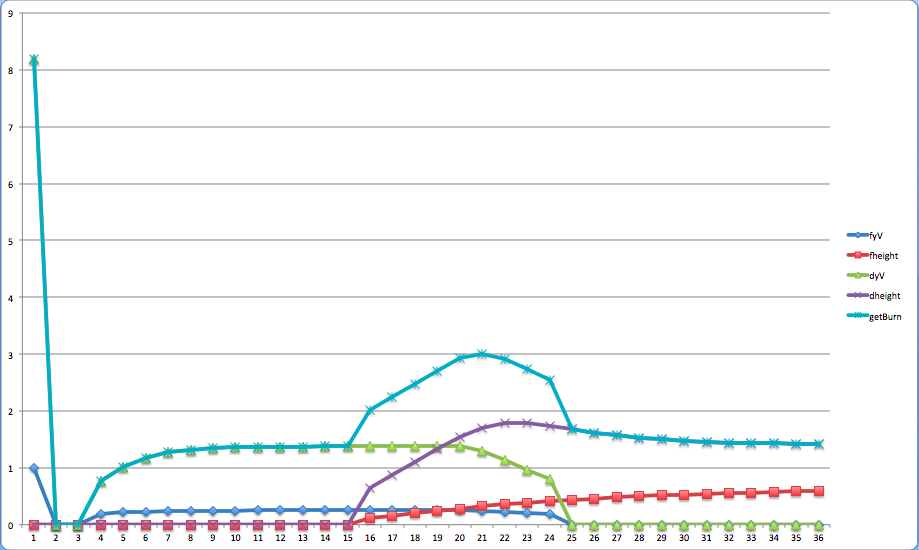
\includegraphics[width=130mm]{report_images/smooth.png}
                \caption{Smooth landing with small overcorrection}
                \label{smooth}
        \end{center}
\end{figure}

\begin{figure}[h!]
        \begin{center}
                \includegraphics[width=130mm]{report_images/low_grav.png}
                \caption{Overcorrection with low gravity}
                \label{smooth}
        \end{center}
\end{figure}

\begin{figure}[h!]
        \begin{center}
                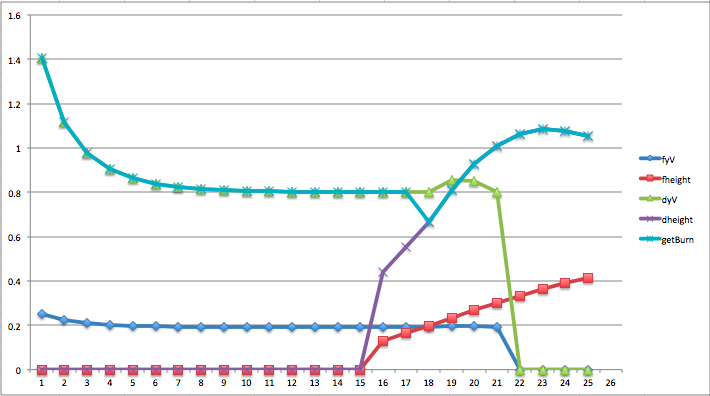
\includegraphics[width=130mm]{report_images/smooth2.png}
                \caption{Smooth landing}
                \label{smooth2}
        \end{center}
\end{figure}

\pagebreak

\subsection{X fuzzy values and defuzzified output with scaling (getThrust)}

\begin{figure}[h!]
        \begin{center}
                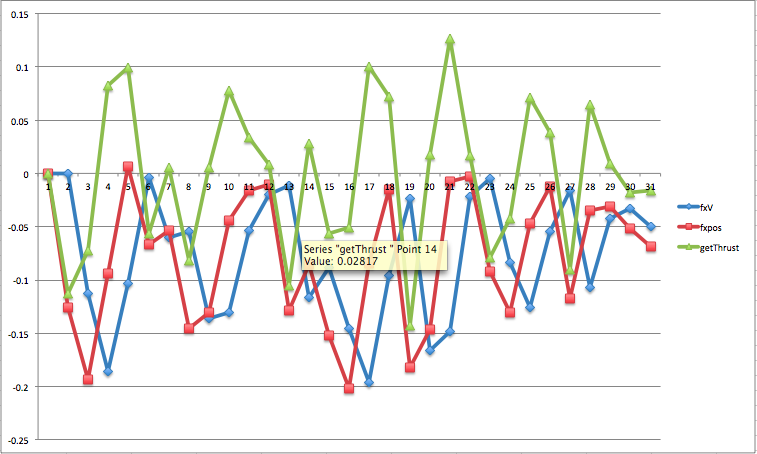
\includegraphics[width=130mm]{report_images/med_wind.png}
                \caption{Medium wind with overcorrection}
                \label{med_wind}
        \end{center}
\end{figure}

\pagebreak

\begin{figure}[h!]
        \begin{center}
                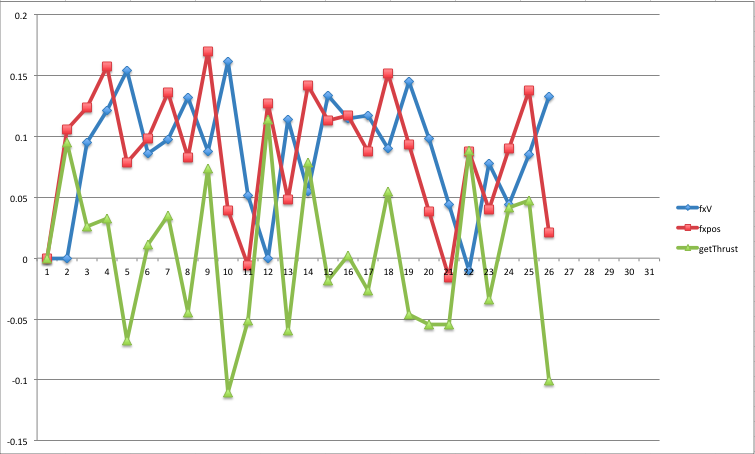
\includegraphics[width=130mm]{report_images/low_wind.png}
                \caption{Low wind}
                \label{low_wind}
        \end{center}
\end{figure}

\begin{figure}[h!]
        \begin{center}
                \includegraphics[width=130mm]{report_images/crash2.png}
                \caption{Crash!}
                \label{low_wind}
        \end{center}
\end{figure}


\end{document}
